\documentclass[11pt]{article}
\usepackage[T1]{fontenc}      % proper glyphs (<, >, |) and hyphenation
\usepackage{lmodern}
\usepackage[margin=1in]{geometry}
\usepackage{graphicx}\graphicspath{{figures/}}
\usepackage{booktabs}
\usepackage{tabularx}
\usepackage{microtype}
\usepackage{xcolor}
\usepackage{hyperref}
\usepackage{xurl}              % break long URLs at safe characters
\usepackage[htt]{hyphenat}    % allow breaks inside \texttt{} (file paths)
\sloppy                        % prefer loose spacing over right-margin overflow
\emergencystretch=3em          % last-resort stretch for unbreakable lines
% PPI theme -- Progress and Poverty Institute brand styling.
% Colors sampled from progressandpovertyinstitute.org (indigo family + coral accent).
% Requires xcolor (loaded in the main preamble) and hyperref.
\definecolor{ppiprimary}{HTML}{475BB2}  % indigo (primary brand)
\definecolor{ppidark}{HTML}{2D3559}     % deep navy
\definecolor{ppilight}{HTML}{579AF6}    % sky accent
\definecolor{ppiaccent}{HTML}{FF4F55}   % coral accent
\usepackage{sectsty}
\allsectionsfont{\color{ppidark}}
\hypersetup{colorlinks=true,linkcolor=ppiprimary,urlcolor=ppiprimary,citecolor=ppiprimary}


% Generated headline numbers — produced by paper/scripts/generate_paper_assets.py.
% Run that generator BEFORE writing/compiling prose; never type result numbers here.
\InputIfFileExists{tables/headlines.tex}{}{}

\begin{document}

\begin{center}
  \IfFileExists{figures/ppi-logo.png}{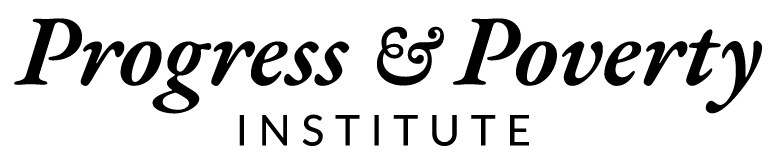
\includegraphics[height=1.3cm]{ppi-logo}\\[0.7em]}{}
  {\LARGE\bfseries\color{ppiprimary} Who Owns Philadelphia's Vacant Land?\par}
  \vspace{0.4em}
  {\large\itshape Ownership, absentee capital, and who would pay under a land value tax\par}
  \vspace{0.9em}
  {\large Russell Richie\par}
  \vspace{0.2em}
  {\normalsize Progress and Poverty Institute\par}
  \vspace{0.2em}
  {\normalsize \today\par}
\end{center}
\vspace{0.8em}

\begin{abstract}
\noindent
The case for taxing land in Philadelphia usually comes with a villain: the absentee
speculator sitting on a vacant lot, waiting for someone else's investment to raise its
price. This report tests that story against the assessor's own ownership records for all
\PhilOwnTotalParcels{} parcels in tax year~\PhilOwnTaxYear{}, and finds it half right.
Vacant land really is investor-held in a way housing is not: LLCs hold
\PhilOwnVacantLlcShare{} of privately owned vacant land value against
\PhilOwnSfrLlcShare{} for single-family homes, a \PhilOwnVacantVsSfrRatio{} gap. But those
LLCs are mostly \emph{local}. Only \PhilOwnVacantLlcOos{} of LLC-owned vacant land value
belongs to owners who receive their mail out of state --- below the citywide LLC average of
\PhilOwnCityLlcOos{}, and far below commercial property at \PhilOwnCommercialLlcOos{}.
Vacant land is also not the most investor-held property type in the city; it ranks
\PhilOwnVacantLlcRank{}th of \PhilOwnTaxableCategories{}, behind industrial land
(\PhilOwnIndustrialLlcShare{}), large multi-family (\PhilOwnLargeMfLlcShare{}), and ordinary
commercial property (\PhilOwnCommercialLlcShare{}). Under a revenue-neutral 4:1 split-rate
reform, LLC owners of vacant land and parking would pay \PhilOwnVpLlcTaxChangeM{} more per
year. The policy case for the reform survives all of this; the rhetorical case for
\emph{out-of-state} villains does not, and a campaign that leads with it is picking the one
claim the data will not support.
\end{abstract}

\section{The question}

An advocate arguing for a land value tax in Philadelphia has a story ready to hand. The city
has tens of thousands of vacant parcels, disproportionately in disinvested neighborhoods;
somebody owns them; that somebody is presumed to be an investor waiting for appreciation
rather than a neighbor. Shift the tax onto land, the argument goes, and the holding cost of
speculation rises until the lots get built or sold.

The mechanism does not actually require a villain --- an idle lot imposes the same cost on a
neighborhood whoever holds the deed. But the politics tend to want one, and the specific
villain reached for is usually the out-of-town speculator. That is an empirical claim, and
Philadelphia publishes enough data to check it. This report asks three questions of the
assessor's records: who owns each type of property in Philadelphia, where do those owners
receive their mail, and who would pay more under the reform.

\section{Data and methods}

The universe is every parcel in the Office of Property Assessment's tax-year~\PhilOwnTaxYear{}
roll --- \PhilOwnTotalParcels{} parcels --- joined to the LVTShift model's per-parcel tax
results for a revenue-neutral 4:1 split-rate reform. Ownership comes from two OPA fields: the
recorded owner name, and the owner's mailing address.

\paragraph{Owner type.} Owner names are classified by legal form --- LLC, LP/LLP,
corporation, trust or estate, other business, or individual --- from the name string.
Business names sharing a mailing address are then unioned into a single \emph{entity}, so
that a landlord operating through a dozen single-purpose LLCs at one office counts once.
Individuals are deliberately \emph{not} merged by address: doing so chains condominium towers
and management offices into fictitious mega-owners. Every share reported below is a share of
land value unless stated otherwise, and public agencies (the City, the Land Bank, the
Redevelopment Authority, PHA, SEPTA, the Commonwealth) are excluded from the private
denominator and reported separately.

\paragraph{Owner location.} Mailing addresses are bucketed as in-city, suburban
Pennsylvania, the NJ/DE metro, or out-of-state. This is a location proxy, not beneficial
ownership --- see Section~\ref{sec:caveats}.

\paragraph{Property type.} Categories are the model's own, with one correction. OPA assigns
most surface parking lots the same use code as vacant land, so parking sits invisibly inside
``vacant land'' in the raw roll. The \texttt{R*} building-code family separates it, and
parking is broken out here into \PhilOwnParkingCategories{} categories. Vacant land and
parking together --- the categories a land value tax hits hardest --- account for
\PhilOwnVpParcels{} parcels, of which \PhilOwnVpPrivateParcels{} are privately owned. Only
\PhilOwnVpPublicParcels{} (\PhilOwnVpPublicShare{}) are held by public agencies, because most
publicly owned vacant land is fully exempt and sits outside the taxable universe entirely.
Any claim about ``who owns the vacant land'' that includes exempt public holdings is
answering a different question than the one about who pays.

\section{Results}

\subsection{Vacant land is investor-held relative to housing --- and ordinary relative to
everything else}

The first half of the advocate's story holds up. LLCs hold \PhilOwnVacantLlcShare{} of
privately owned vacant land value, against \PhilOwnSfrLlcShare{} for single-family homes: a
\PhilOwnVacantVsSfrRatio{} gap, and the widest contrast in the data. Counting every business
form rather than LLCs alone, \PhilOwnVacantBusinessShare{} of private vacant land value is
held by a business entity.

But vacant land is not exceptional among \emph{non-residential} property. Figure~\ref{fig:share}
and Table~\ref{tab:share} rank all \PhilOwnTaxableCategories{} taxable property types by LLC
share; vacant land comes \PhilOwnVacantLlcRank{}th. Industrial land
(\PhilOwnIndustrialLlcShare{}), large multi-family buildings (\PhilOwnLargeMfLlcShare{}), and
ordinary commercial property (\PhilOwnCommercialLlcShare{}) are all more LLC-held. Surface
parking, often paired with vacant land in the same argument, is lower still ---
\PhilOwnParkingCommLlcShare{} for commercial lots, \PhilOwnParkingNoncommLlcShare{} for
non-commercial, \PhilOwnGarageLlcShare{} for structured garages. What is distinctive about
vacant land is the gap against \emph{housing}, not against commercial property generally. A
campaign claiming vacant lots are uniquely investor-held is overstating a real but narrower
fact.

\begin{figure}[htbp]
  \centering
  \includegraphics[width=\linewidth]{llc_share.pdf}
  \caption{LLC share of privately owned land value, by property type. Vacant land and
  parking are highlighted. Numbers at the right of each bar are private parcel counts --- a
  share over nine parcels should not read like a share over twenty-eight thousand.}
  \label{fig:share}
\end{figure}

\begin{table}[htbp]
  \centering
  \caption{Ownership by property type. ``LLC (upper)'' is the truncation-corrected upper
  bound described in Section~\ref{sec:caveats}; ``any business'' includes corporations,
  partnerships, and trusts.}
  \label{tab:share}
  \small
  \input{tables/llc_share.tex}
\end{table}

\subsection{Individuals own most vacant parcels}

Within taxable vacant land, individuals hold \PhilOwnVacantIndividualParcels{} parcels
against \PhilOwnVacantBusinessParcels{} held by business entities
(Table~\ref{tab:vacantsector}). Individuals own more \emph{parcels}; businesses own slightly
more \emph{value} --- \PhilOwnVacantBusinessLandShare{} against
\PhilOwnVacantIndividualLandShare{}. ``Vacant lots are owned by speculators'' is true of the
dollars and false of the parcel count. It is also worth noticing where the tax falls:
individuals holding vacant land would pay nearly as much more in aggregate as business
entities would. Messaging that implies only speculators pay will not survive a reporter
pulling ten addresses at random.

\begin{table}[htbp]
  \centering
  \caption{Who owns vacant land, and who pays. Shares are of all vacant land value including
  publicly owned parcels, which is why the private-only figures quoted in the text differ
  slightly.}
  \label{tab:vacantsector}
  \small
  \input{tables/vacant_sector.tex}
\end{table}

\subsection{The absentee story runs the other way}
\label{sec:absentee}

Across all \PhilOwnCategories{} property categories, LLC owners really are more absentee than
owners generally: \PhilOwnCityLlcOos{} of LLC-owned land value belongs to out-of-state
owners, against \PhilOwnCityAllOos{} for private owners as a whole, and only
\PhilOwnCityLlcIncity{} of LLC land value is held in-city against \PhilOwnCityAllIncity{}
overall. So the instinct that entity ownership travels with absentee ownership is correct as
a general matter.

But it does not hold for the categories a land value tax targets. Figure~\ref{fig:scatter} is
the central result of this report: it plots each property type by how LLC-held it is against
how out-of-state those LLC owners are, and the two do not move together. Vacant land sits at
\PhilOwnVacantLlcOos{} out-of-state --- \emph{below} the citywide LLC average, and only
modestly above single-family housing at \PhilOwnSfrLlcOos{}. The genuinely absentee
categories are elsewhere: commercial property at \PhilOwnCommercialLlcOos{}, and structured
parking garages and hotels higher still (Figure~\ref{fig:geography},
Table~\ref{tab:geography}). Taking vacant land and parking together, LLC owners are
\PhilOwnVpLlcIncityShare{} in-city by land value and \PhilOwnVpLlcOosShare{} out-of-state; of
\PhilOwnVpLlcEntities{} distinct LLC entities, \PhilOwnVpLlcIncityEntities{} mail to a
Philadelphia address and \PhilOwnVpLlcOosEntities{} mail out of state.

The uncomfortable implication for messaging is specific: ``out-of-state speculators are
sitting on our vacant lots'' is the one version of the claim the data does not support.
``Absentee owners hold our commercial land'' is much better supported --- but that is an
argument for a different reform, aimed at a different constituency.

\begin{figure}[htbp]
  \centering
  \includegraphics[width=\linewidth]{absentee_scatter.pdf}
  \caption{Investor-held does not mean absentee. Each point is a property type; marker size
  scales with total private land value. Vacant land and parking (coral) sit at or below the
  citywide LLC out-of-state average, while commercial property, garages, and industrial land
  sit well above it.}
  \label{fig:scatter}
\end{figure}

\begin{figure}[htbp]
  \centering
  \includegraphics[width=\linewidth]{llc_geography.pdf}
  \caption{Where LLC owners receive their mail, by property type, as a share of LLC-owned
  land value. Ordered most to least out-of-state.}
  \label{fig:geography}
\end{figure}

\begin{table}[htbp]
  \centering
  \caption{Owner mailing address by property type: all private owners against LLC owners
  only. The LLC columns are a subset of the all-owner columns, which is why LLC shares are
  systematically more distant.}
  \label{tab:geography}
  \small
  \input{tables/geography.tex}
\end{table}

\subsection{The out-of-state owners who do exist are few, large, and real}

Out-of-state ownership is small here, but it is genuine rather than a registered-agent
artifact --- a confound that contaminates this kind of analysis often enough to be worth
ruling out explicitly. In the whole vacant-and-parking set, exactly
\PhilOwnDelawareParcels{} parcels mail to Delaware --- the state whose registered-agent
industry usually shows up first in an ownership file. The out-of-state parcels spread across
\PhilOwnOosAddresses{} distinct
mailing addresses with at most \PhilOwnOosMaxNames{} different LLC names sharing any one of
them; citywide across all property types it is \PhilOwnCityOosAddresses{} addresses with at
most \PhilOwnCityOosMaxNames{} names at any one. Registered-agent hubs look like dozens of
names at a single address, and neither scope shows that pattern.

What the out-of-state holdings do show is concentration: the top \PhilOwnOosTopN{} mailing
addresses hold \PhilOwnOosTopTenShare{} of out-of-state LLC land value, with the largest
single address in \PhilOwnTopOosCity{}. The honest formulation is a small number of large
out-of-town institutional owners, and a much larger number of local LLCs.

Figure~\ref{fig:map} shows the same thing geographically. Vacant land and parking cluster
heavily in North and West Philadelphia, and LLC ownership tracks that footprint rather than
concentrating in the high-value core; out-of-state parcels are scattered thinly across it
rather than massed anywhere in particular.

\begin{figure}[htbp]
  \centering
  \includegraphics[width=\linewidth]{map.pdf}
  \caption{Privately owned vacant land and parking parcels (left), and the LLC-owned subset
  with out-of-state owners highlighted (right). Local and out-of-state markers are drawn at
  near-equal size deliberately; enlarging the minority category would overstate it.}
  \label{fig:map}
\end{figure}

\subsection{Many small owners, concentrated value}

Restricting to vacant land alone, \PhilOwnVacantEntities{} distinct LLC entities hold
\PhilOwnVacantEntityParcels{} parcels worth \PhilOwnVacantEntityLandM{} in land value. The
portfolio structure cuts against the assembler stereotype:
\PhilOwnVacantSingleParcelEntityShare{} of these entities own exactly one vacant parcel, and
those single-parcel owners account for \PhilOwnVacantSingleParcelLandShare{} of the value.
Only \PhilOwnVacantBigEntities{} entities hold fifty or more vacant parcels, together just
\PhilOwnVacantBigLandShare{} of the value.

But the value itself is highly concentrated, and that is a different axis from portfolio size
(Figure~\ref{fig:concentration}, right panel). The largest holders in Table~\ref{tab:entities}
are mostly \emph{single-parcel} development sites, not land banks --- the top entry is one
lot. Concentration in this market is in dollars, not in deed counts, and a policy aimed at
breaking up large portfolios would miss most of the value.

\begin{figure}[htbp]
  \centering
  \includegraphics[width=\linewidth]{vacant_concentration.pdf}
  \caption{Vacant-land LLC entities by portfolio size (left) and the Lorenz curve of land
  value across entities (right). Most entities own one parcel; most value sits with a few.}
  \label{fig:concentration}
\end{figure}

\begin{table}[htbp]
  \centering
  \caption{The \PhilOwnVacantTopEntityShown{} largest LLC entities by vacant land value.
  ``Names'' is the number of distinct assessor owner strings unioned into the entity; owner
  strings are reproduced as the assessor records them. Rows with many names and many parcels
  should be read with the entity-resolution caveat in Section~\ref{sec:caveats}.}
  \label{tab:entities}
  \small
  \input{tables/top_entities.tex}
\end{table}

\subsection{Who pays}

Under the modelled revenue-neutral 4:1 split-rate reform, LLC owners of vacant land and
parking pay \PhilOwnVpLlcTaxChangeM{} more per year across \PhilOwnVpLlcParcels{} parcels.
Figure~\ref{fig:taxshift} breaks the shift down by owner type within each headline category.
The pattern to notice is that business entities and individuals both carry a large share of
the increase on vacant land --- consistent with individuals holding more vacant parcels than
businesses do.

\begin{figure}[htbp]
  \centering
  \includegraphics[width=\linewidth]{tax_shift.pdf}
  \caption{Change in annual tax bills under the reform, by owner type, for vacant land and
  each parking category.}
  \label{fig:taxshift}
\end{figure}

\begin{figure}[htbp]
  \centering
  \includegraphics[width=\linewidth]{owner_sector.pdf}
  \caption{Composition of each property type by owner type, as a share of land value.}
  \label{fig:sector}
\end{figure}

\section{Caveats}
\label{sec:caveats}

\paragraph{Every LLC share here is a floor.} Hand-adjudication of a
\PhilOwnClassifierSample{}-name sample puts LLC precision at \PhilOwnLlcPrecision{} --- no
false positives (Table~\ref{tab:precision}). Separately, OPA truncates owner names at
\PhilOwnTruncationWidthOne{} and \PhilOwnTruncationWidthTwo{} characters, which cuts the
legal suffix off longer names and pushes entities \emph{out} of the LLC bucket, never into
it; the ``other business'' bucket is correspondingly the least precise at
\PhilOwnOtherBusinessPrecision{}. The ``LLC (upper)'' column in Table~\ref{tab:share}
reallocates truncated names at the LLC rate observed among untruncated ones, which lifts
vacant land from \PhilOwnVacantLlcShare{} to \PhilOwnVacantLlcShareUpper{}. Note also that
LLC ownership is more common by value than by parcel: \PhilOwnVacantLlcParcelShare{} of
private vacant \emph{parcels} are LLC-held, against \PhilOwnVacantLlcShare{} of value.

\paragraph{Mailing address is a location proxy, not beneficial ownership.} An out-of-state
address may belong to an accountant acting for a Philadelphian; a Philadelphia address may
front an entity owned elsewhere. True beneficial ownership is not obtainable at scale by any
route --- the FinCEN beneficial-ownership registry is not public and is exempt from FOIA, and
its reporting requirement for domestic companies was narrowed in 2025. Tracing owners through
Pennsylvania Department of State filings and deeds is feasible by hand for the largest
holders only. The absentee findings in Section~\ref{sec:absentee} should be read as claims
about where owners receive mail, which is what the assessor knows.

\paragraph{Concentration figures are lower bounds.} Entity resolution unions business names
sharing a mailing address, but shell networks registered at different addresses under
unrelated names remain unresolved. In the other direction, a shared-address union can
over-merge: the rows in Table~\ref{tab:entities} with many constituent names and many parcels
are the ones most likely to be an address hub rather than a single owner, and are worth
checking individually before citing.

\paragraph{The vacant-land universe is the assessor's, which is what the tax bills.} It
agrees reasonably with the City's 2025 Land Use layer (Jaccard \PhilOwnJaccardVacantLandUse{})
and with L\&I's Vacant Indicators (\PhilOwnJaccardVacantLandI{}). The parking universe does
\emph{not} agree with the Land Use layer (\PhilOwnJaccardParkingLandUse{}) --- that layer
identifies only \PhilOwnCountParkingLandUse{} parking parcels citywide against the assessor's
\PhilOwnParkingOpaCount{}, so it under-identifies surface parking badly and is not usable as
a source. The assessor codes are corroborated instead by an independent OPA extract at
Jaccard \PhilOwnJaccardParkingOpa{} (Table~\ref{tab:universe}).

\paragraph{Land values are OPA's.} Re-running the headline shares on the LYCD
location-value model moves the vacant-land LLC share by \PhilOwnRobustVacantDiffPp{}. The
largest divergence in any category is \PhilOwnRobustMaxDiffPp{}, for
\PhilOwnRobustMaxCategory{} --- a small category where either land-value model is doing a
lot of work. The headline comparisons are not sensitive to this choice; the parking-garage
figures are.

\begin{table}[htbp]
  \centering
  \caption{Classifier precision by predicted owner form, hand-adjudicated.}
  \label{tab:precision}
  \small
  \input{tables/precision.tex}
\end{table}

\begin{table}[htbp]
  \centering
  \caption{Agreement between this study's universes and independent sources.}
  \label{tab:universe}
  \small
  \input{tables/universe.tex}
\end{table}

\section{What this means for the campaign}

Three things follow, and they are not the three an advocate would pick in advance.

First, the strongest ownership fact available is a comparison, not an accusation: vacant land
is \PhilOwnVacantVsSfrRatio{} more investor-held than the housing stock. That contrast is
robust, it is large, and it makes the point that a land value tax reaches a kind of holding
that ordinary homeowners are not doing.

Second, the absentee framing should be retired for vacant land specifically. At
\PhilOwnVacantLlcOos{} out-of-state --- below the citywide LLC average --- an opponent can
refute ``out-of-state speculators'' with the assessor's own file in an afternoon, and the
refutation would be correct. The version of the claim that survives is narrower and duller:
the owners are disproportionately entities rather than households, and they are mostly from
here.

Third, and least comfortable: a substantial share of the increase on vacant land falls on
individuals, not investors. A campaign that promises otherwise is setting up its own
counter-story. The better argument does not depend on who holds the deed. An idle lot
withholds the same site from the same neighborhood regardless of whether its owner lives in
Fishtown or Fort Lauderdale, and the reform's case is that the holding cost should reflect
that. Philadelphia will not get many clean shots at this; the argument it leads with should
be the one that does not break on contact with the data.

\paragraph{Reproducibility.} Every number, table, and figure in this report is generated by
\texttt{paper/scripts/generate\_paper\_assets.py} from the tracked outputs of
\texttt{ownership\_by\_type.py}; no value is typed into the prose. Regenerate the assets and
rebuild the PDF with a single command each after any change to the analysis.

\end{document}
